
\section{Case study}
\label{sec:sysml}
To illustrate our approach, we take an example (water tank) inspired by \cite{AmalioPCW16}. According to the I/O dependency information between the FMUs, the architectural model for water tank is constructed using SysML. The aim of using SysML is to design the architecture of the system with a more high-level modeling language. It helps to show the components and their connection.

%\subsection{Case Study: Water Tank}

The water tank system is our running example. A source of water flows into the water tank whose water flows into the drain, and the source is controlled by a valve; when the valve is open the water flows into the water tank. The valve, managed by a software controller, is opened or closed stochastically or depending on the water level. There are two variants of water tank system depending on the various connections between controller, valve and tank. 

\subsection{Architecture Modelling in SysML}
SysML is a general purpose domain-specific language (DSL) \cite{SemerathBHSV17} for model-based systems engineering (MBSE) \cite{Dori16}, which is originated as an initiative of the International Council on Systems Engineering (INCOSE) \cite{Pepper2015International} in January 2001. SysML is implemented as a UML profile. The \textit{Block Definition Diagram }(BDD) describes the system blocks and their features (structural and behavioural). The\textit{ Connection Diagram} (CD) describes the internal structure of blocks. The ports of blocks are connected by the connector. The I/O dependence of blocks describes the communication between blocks. SysML block diagrams are usually used to describe the architecture of systems.

Figure~\ref{myad} shows the block definition diagram for the water tank system. The system consists of three blocks, i.e., \emph{Valve}, \emph{Tank} and \emph{Controller}, in which \emph{Valve} and \emph{Tank} are physical components. \emph{Controller} is the cyber component. Each component has its own input and output. For instance, the input interface of \emph{Valve} is named as \emph{vin}, which is used to input the \emph{Open-Closed} signal. 
\begin{figure}[htbp]
	\centering	{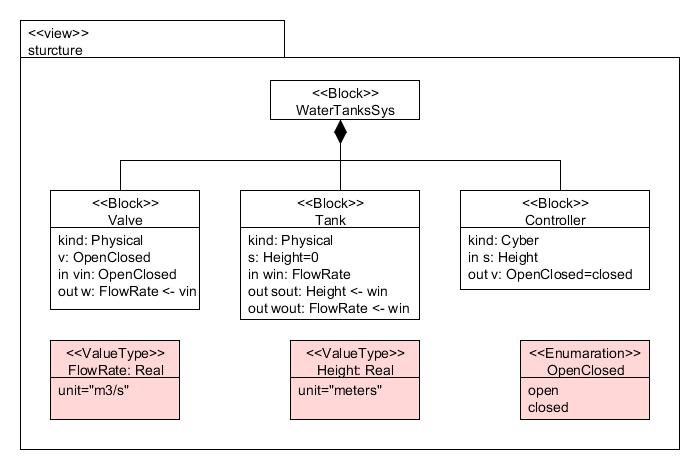
\includegraphics[width=3.2in,height=2.3in]{fig/AD.jpg}}
	\caption{SysML BDD for water tank system.}
	\label{myad}
\end{figure}
Figure~\ref{cd} shows the connection diagram for the system. There are three cases for connections. The first case is that the system has one valve, one controller and one tank. The controller sends stochastic signals to control the valve on/off leading to various rate of water flow. The second case is that the signal from the controller is affected by the water level of the tank. The last case is on the basis of the first case and adds another tank2 which is affected by the flow rate of the tank1.

\begin{figure}[htbp]
\centering{
		\subfigure[Connection case 1]{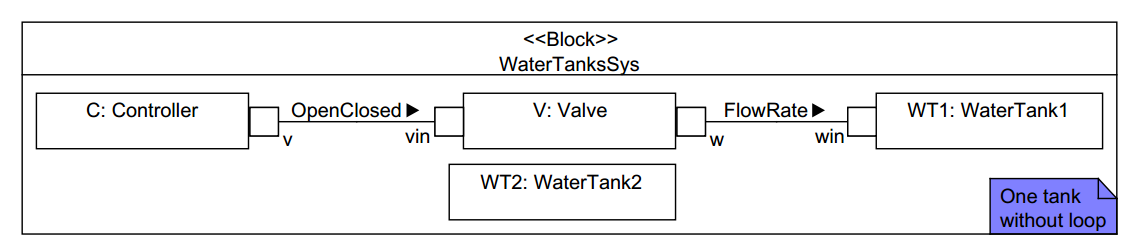
\includegraphics[width=3.2in,height=0.8in]{fig/CD1.png}
			\label{cd1}}
		\hfil
		\subfigure[Connection case 2]{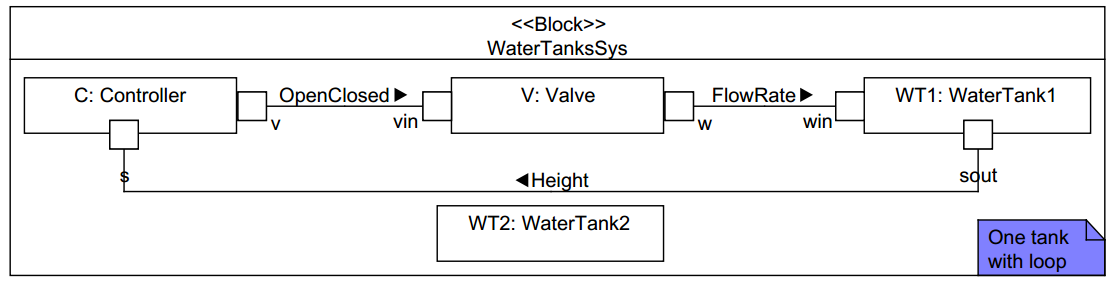
\includegraphics[width=3.2in,height=0.8in]{fig/CD2.png}
			\label{cd2}}
		\hfil
		\subfigure[Connection case 3]{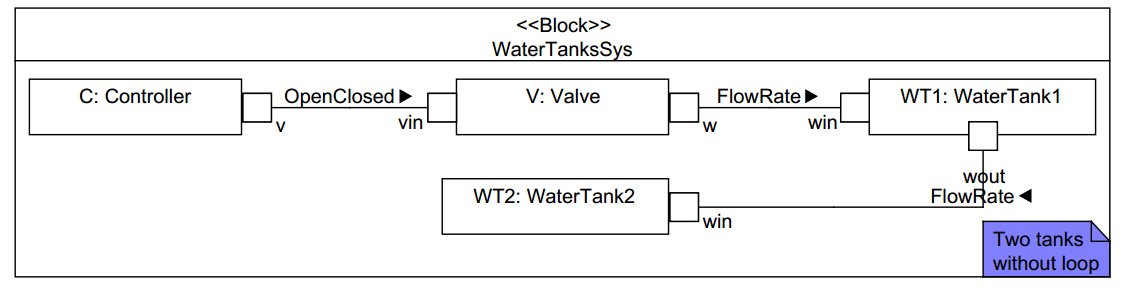
\includegraphics[width=3.2in,height=0.8in]{fig/CD3.png}
			\label{cd3}}
	\caption{SysML CD for water tank system.}
	\label{cd}
	}
\end{figure}
We model the architecture with SysML which is a high-level modeling language. The SysML BDD shows the blocks of system and SysML CD shows the connection between blocks. In next section, we abstract each block as a FMU, and obtain the connection between based on the SysML CD.

\subsection{The FMUs  Connection of Water Tank System}
Figure~\ref{fmu-con} is the FMUs and FMUs connection of water tank system. There are three connection cases between the FMUs according to the SysML CD in the previous section. The first case contains three FMU components (\emph{Controller}, \emph{Valve} and \emph{ Tank1}) and two channels($v \_ vin$, $w \_ win$) as shown in Fig.\ref{fmu-con1}. The controller and valve are connected with channel $v \_ vin$. The valve and tank1 are connected with channel $w \_ win$. The second case is shown in Fig.\ref{fmu-con2}, there could be a channel $sout \_ s$ between tank1 and controller, which means the water level of tank1 affecting the control strategy of the controller. Figure~\ref{fmu-con3} shows the third case, there could be another (tank2). The tank1 and tank2 are connected by the channel $w \_ out$. 
\begin{figure}[htbp]
\centering{
		\subfigure[Connection case 1]{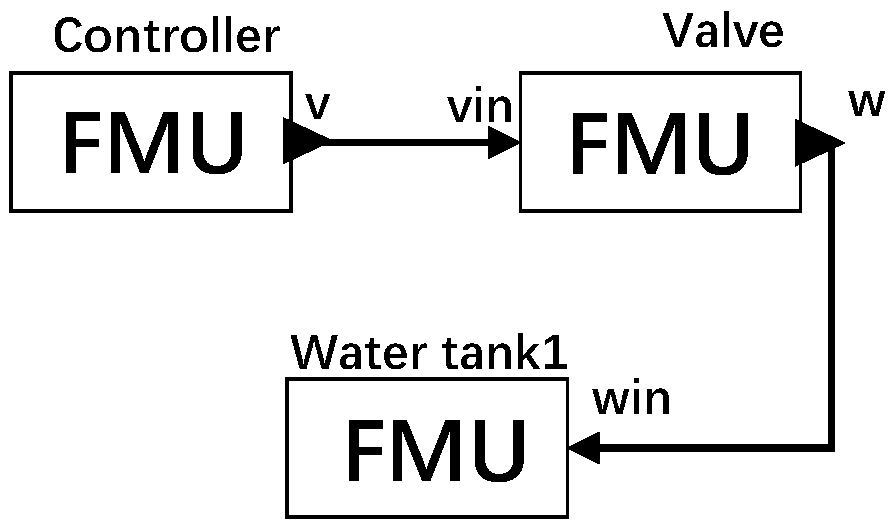
\includegraphics[width=1.0in,height=0.6in]{fig/fmuc1.png}
			\label{fmu-con1}}
		\hfil
		\subfigure[Connection case 2]{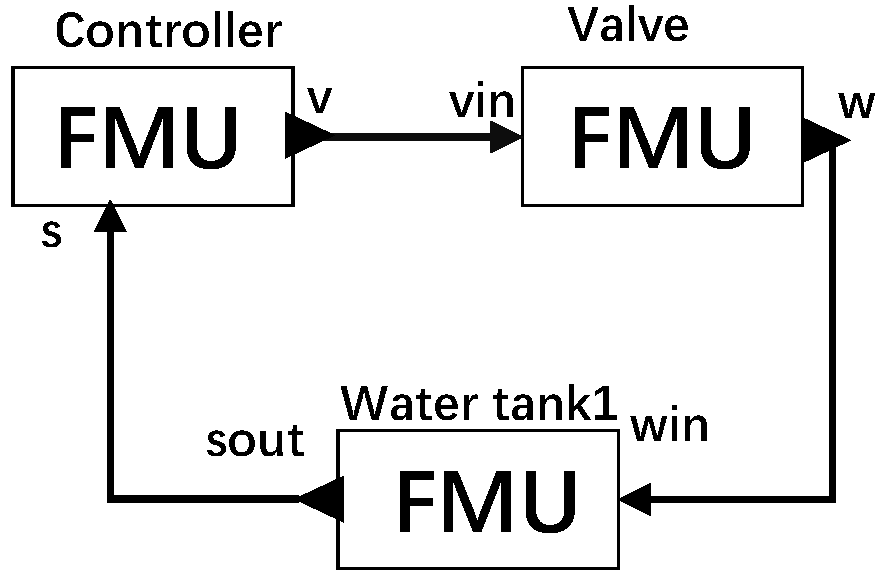
\includegraphics[width=1.0in,height=0.6in]{fig/fmuc2.png}
			\label{fmu-con2}}
		\hfil
		\subfigure[Connection case 3]{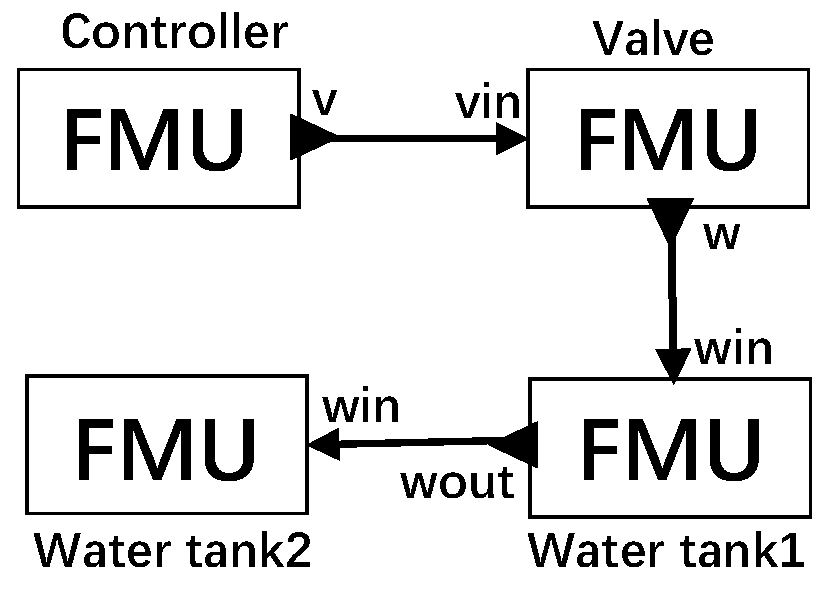
\includegraphics[width=1.0in,height=0.6in]{fig/fmuc3.png}
			\label{fmu-con3}}
	\caption{FMUs connection of water tank system.}
	\label{fmu-con}
	}
\end{figure}
How can we assure the correctness of the architecture models? We attempt to verify it with model checking based on timed automata. More details on verification process can be found in the next section.